Sowohl das Black-Box-Problem als auch Überanpassung der Algorithmen stellen Hindernisse für die Zulassung von Medizinprodukte mit KI dar. Zulassungsstellen haben Schwierigkeiten zu bestimmen, wie und ob die Algorithmen funktionieren und ob ihre Erkennungsleistung auch auf andere Datensätze angewandt werden kann \cite{AI_where_are_we_now}.\\
Zur Lösung des Black-Box-Problems wurde in unterschiedlichen Studien eine Heatmap erstellt, um Regionen mit erhöhter Aktivierung des Deep Learning Netzwerks grafisch darzustellen. Man schloss daraus, dass es sich bei stark aktivierten Bereichen um Regionen handelt, die für die Bestimmung der Diagnose entscheidend sind \cite{AI_where_are_we_now}.
\begin{figure}[h]
    \centering
    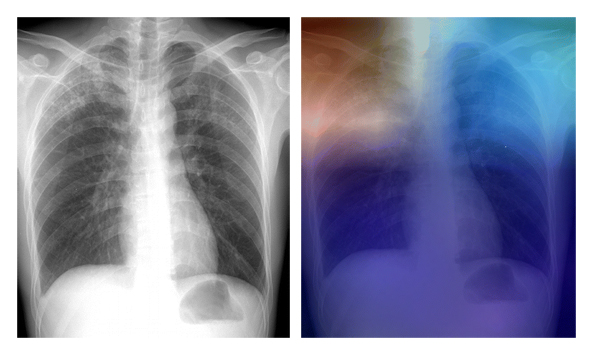
\includegraphics[width=0.6\textwidth]{images/heatmap.jpg}
    \caption{\label{fig:Heatmap}
        Links Röntgenbild, Rechts Heatmap 
        \protect\cite{AI_where_are_we_now}
    }
\end{figure}\\
Auch für die Überanpassung von KI Algorithmen gibt es bereits Ansätze: Algorithmen werden nach dem Training an verschiedenen Datensätzen getestet\cite{AI_where_are_we_now} und die Ergebnisse grafisch in Form einer Area Under the Curve (AUC) Kurve dargestellt. Bei einem Algorithmus, der an einer Übereinpassung leidet, würde man erwarten, dass seine Genauigkeit, gemessen mit der AUC, bei Datensätzen, die nicht den gleichen Ursprung haben wie die Trainingsdaten, deutliche schlechter ist \cite{AI_where_are_we_now}.\\
Das Potential der KI überwiegt in der Medizin  gegenüber den Risiken und Grenzen  \cite{Chapter_14}. Trotz bestehender Lösungen für das Black-Box-Problem und Überanpassungen der KI Algorithmen ist es weiterhin unumgänglich, den Mensch in die Entscheidung miteinzubeziehen und Interaktionen zwischen dem KI-System und dem Mensch zu ermöglichen
\cite{AI_where_are_we_now}.
